%!TEX encoding = UTF-8 Unicode
%!TEX root = ../fiche.tex

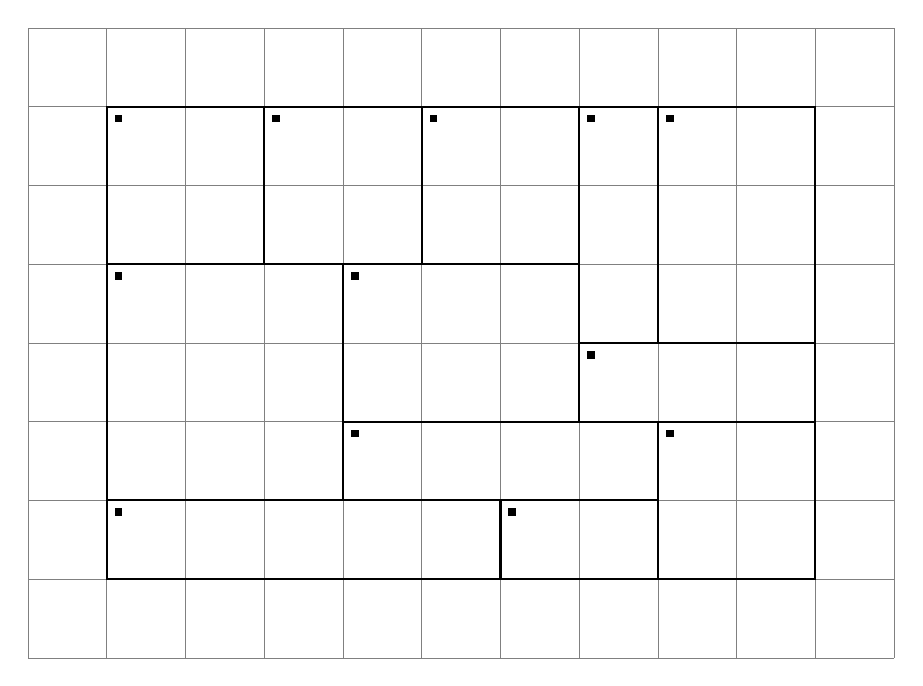
\begin{tikzpicture}

% define base units ------------------------------------------------------------
	\def\delta{1/10}

% draw grid --------------------------------------------------------------------
	\draw[step=1, gray, very thin] (-1,-1) grid (10,7);

% draw rectangles --------------------------------------------------------------
	\def\rect{
%		coord_x / coord_y / size_x /size_y
		0 / 0 / 5 / 1,
		0 / 1 / 3 / 3,
		0 / 4 / 2 / 2,
		2 / 4 / 2 / 2,
		3 / 1 / 4 / 1,
		3 / 2 / 3 / 2,
		4 / 4 / 2 / 2,
		5 / 0 / 2 / 1,
		6 / 2 / 3 / 1,
		6 / 3 / 1 / 3,
		7 / 0 / 2 / 2,
		7 / 3 / 2 / 3
	}
	\foreach \x / \y / \sx / \sy in \rect
	{
		\draw[thick] (\x,\y) rectangle +(\sx,\sy);
		\fill (\x+\delta,\y+\sy-\delta) rectangle +(\delta,-\delta);
	}

\end{tikzpicture}
